\documentclass[12pt]{article}
\usepackage{setspace}
\usepackage{extsizes}
\usepackage{float}
\usepackage{amsmath, amsthm, amssymb}    
\usepackage[margin=.5in]{geometry}
\usepackage{tikz}
\usepackage{pgfplots}
\pgfplotsset{compat=1.13}
\usepackage{tkz-euclide}
\usepackage{graphicx}


\title{\vspace{-2.0cm}Homework 9}
\author{Joanne Wardell}
\date{Tuesday, October 2, 2018}
\begin{document}
\maketitle

\subsection*{Section 14.7}
\noindent 2.) $f(x,y) = 2xy-5x^{2}-2y^{2}+4x + 4y -4$\\\\
\noindent $\frac{\partial f}{\partial x} = -8x + 4$, \hspace{10pt} $\frac{\partial ^{2} f}{\partial x^{2}} = -8$\\\\
\noindent $\frac{\partial f}{\partial y} = -2y + 4$, \hspace{10pt} $\frac{\partial ^{2} f}{\partial y^{2}} = -2$\\\\
\noindent $\frac{\partial^{2} f}{\partial x \partial y } = \frac{\partial }{\partial x}[-2y + 4] = 0$\\\\
\noindent $\mathbf{H} = f_{xx}f_{yy} - f_{yx}^{2} = 16 > 0$\\\\
\noindent $-8x + 4 = 0 \rightarrow x = 2$\\\\
\noindent $-2y + 4 = 0 \rightarrow y = 2$\\\\
\noindent $f(2, 2) = -8$ is a \textbf{local maximum} since $f_{x}(2, 2) > 0$, $f_{y}(2, 2) > 0$, and $\mathbf{H}\Big|_{(2,2)} > 0$.\\\\
\noindent 10.) $f(x, y) = x^{2} + 2xy$\\\\
\noindent $\frac{\partial f}{\partial x} = 2x + 2y$, \hspace{10pt} $\frac{\partial ^{2} f}{\partial x^{2}} = 2$\\\\
\noindent $\frac{\partial f}{\partial y} = 2x$, \hspace{10pt} $\frac{\partial ^{2} f}{\partial y^{2}} = 0$\\\\
\noindent $\frac{\partial^{2} f}{\partial x \partial y } = \frac{\partial }{\partial x}[2x] = 2$\\\\
\noindent $\mathbf{H} = f_{xx}f_{yy} - f_{yx}^{2} = -4 < 0$\\\\
\noindent $2x+2y = 0$\\\\
\noindent $2x=0= 0 \rightarrow x = 0 \rightarrow y = 0$\\\\
\noindent $f(0, 0) = 0$ is a \textbf{saddle point} since $\mathbf{H}\Big|_{(0,0)} < 0$.\\\\
\noindent 14.) $f(x,y) = x^{3}+3xy + y^{3}$\\\\
\noindent $\frac{\partial f}{\partial x} = 3x^{2} + 3y$, \hspace{10pt} $\frac{\partial ^{2} f}{\partial x^{2}} = 6x$\\\\
\noindent $\frac{\partial f}{\partial y} = 3x + 3y^{2}$, \hspace{10pt} $\frac{\partial ^{2} f}{\partial y^{2}} = 6y$\\\\
\noindent $\frac{\partial^{2} f}{\partial x \partial y } = \frac{\partial }{\partial x}[3x + 3y^{2}] = 3$\\\\
\noindent $3x^{2} + 3y = 0 $\\
\noindent $3x^{2} = -3y \rightarrow y = -x^{2}$\\\\
\noindent $3x + 3y^{2} = 0$\\
\noindent $3x + 3(-x^{2})^{2} = 0$\\
\noindent $3x = -3x^{4}$\\
\noindent $x^{-4}[x = -x^{4}]$\\
\noindent $x^{3}[x^{-3} = -1]$\\
\noindent $-1 = x^{3} \rightarrow x = -1$\\\\
\noindent $y = -((-1)^{2}) = -1$\\\\
\noindent $\mathbf{H} = f_{xx}f_{yy} - f_{yx}^{2} = 36 - 9 > 0$\\\\
\noindent $f(-1, -1) = 1$ is a \textbf{local maximum} since $f_{x}(-1, -1) < 0$, $f_{y}(-1, -1) < 0$, and $\mathbf{H}\Big|_{(2,2)} > 0$.\\\\
\noindent 30.) $f(x, y) = \ln(x + y) + x^{2}-y$\\\\
\noindent $\frac{\partial f}{\partial x} = \frac{1}{x+y} + 2x$, \hspace{10pt} $\frac{\partial ^{2} f}{\partial x^{2}} = -\frac{1}{(x + y)^{2}} + 2$\\\\
\noindent $\frac{\partial f}{\partial y} = \frac{1}{x + y} -1 $, \hspace{10pt} $\frac{\partial ^{2} f}{\partial y^{2}} = -\frac{1}{(x + y)^{2}}$\\\\
\noindent $\frac{\partial^{2} f}{\partial x \partial y } = \frac{\partial }{\partial x}[\frac{1}{x+y} -1 ] = -\frac{1}{(x + y)^{2}}$\\\\
\noindent $\frac{1}{x + y} + 2x= 0 $\\
\noindent $\frac{(x + y)}{-2x}[\frac{1}{x + y} = -2x]$\\
\noindent $y = -2x^{-1} - x$\\\\
\noindent $\frac{1}{x + y} = 0$\\
\noindent $\frac{1}{x  -2x^{-1} -x} = 0 \rightarrow x = 0$\\\\
\noindent $y = 0$\\\\
\noindent $\mathbf{H} = f_{xx}f_{yy} - f_{yx}^{2} = 0$\\\\
\noindent Since $\mathbf{H} = 0$, nothing can be concluded about $f(0, 0)$.\\\\
\noindent 32.) $D(x, y) = x^{2} - xy +y^{2} + 1$, \hspace{10pt} $x = 0$, \hspace{10pt} $y = 4$, \hspace{10pt} $y = x$\\\\
\noindent The function D looks like this:\\
\begin{figure}[!h]
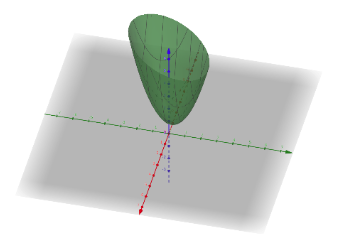
\includegraphics{surface.png}
\end{figure}
\noindent and we are seeking the extreme points enclose within a triangluar area which exists on $D$. We will also search 
for extreme points on the boundaries of this triangular shape. \\\\
\noindent First, we must find the points inside the triangle where there are extremas, aka, when the gradient is $\vec{0}$.\\\\
\noindent $2x - y = 0 \rightarrow y = 2x$\\\\
\noindent $2y - x = 0 \rightarrow x = 0\text{, } y = 0$\\\\
\noindent $\mathbf{point of interest: }D(0,0) = 1$\\\\
\noindent Next, we will test the boundary points by applying three constraints to $D$: the three sides of the triangular shape.\\\\
\noindent $D(0, y) = y^{2} + 1$\\
\noindent $\frac{dD}{dy} = 2y$\\
\noindent $2y = 0 \rightarrow \mathbf{point of interest: } D(0, 0) = 1$\\\\
\noindent $D(x, 4) = x^{2}-4x+17$\\
\noindent $\frac{dD}{dx} =2x -4$\\
\noindent $2x -4 = 0 \rightarrow x = 2$\\
\noindent $\mathbf{point of interest: } D(2, 4) = 13$\\\\
\noindent $D(x, x) = x^{4}+1$\\
\noindent $\frac{dD}{dx} =4x^{3}$\\
\noindent $4x^{3} = 0 \rightarrow x = 0$\\
\noindent $\mathbf{point of interest: } D(0, 0) = 1$\\\\
\noindent Finally, we will exhaust our search by testing the three corners of the triangle.\\\\
\noindent $D(0,0) = 1$, \hspace{10pt} $D(0,4) = 17$, \hspace{10pt} $D(4, 4) = 17$\\\\
\noindent We conclude that within the triangular area, $D$ has an absolute minimum at the origin and absolute maxima at points $(0,4)$ and $(4,4)$.\\\\

\noindent 52.) The minimization of the distance between the point $(2, -1, 1)$ and the plane $x+y-z = 2$ can be obtained as follows.\\\\
\noindent Our goal is to maximize the distance function $f = \sqrt{(x_{1} - x_{0})^{2} + (y_{1} - y_{0})^{2} + (z_{1} - z_{0})^{2}}$\\
\noindent Since $\sqrt{n}$ and $n$, $n \in \mathbb{R}$ are monotonically increasing functions, we can proceed with using $f^{2}$.\\\\
\noindent We have the constrants $g = x+y-z$.\\\\
\noindent We'll evaluate $f$ in the following way: find the distance from the point by evaulating $f$ at the point, but apply the constrains 
that $g$ yeilds. $g$ is a function of two variables which we will solve for $z$. We can interpret $g$ as a $z$ depending on $x$ and $y$, so 
that is the $z$ coordinate we'll restrict $f$ to.\\\\
\noindent $f^{2} = (x-2)^{2} + (y+1)^{2} + (x + y +1)^{2}$\\\\
\noindent  


\subsection*{Section 14.8}
\noindent 2.) $$\\\\
\noindent 4.) $$\\\\
\noindent 8.) $$\\\\
\noindent 24.) $$\\\\
\noindent 26.) $$\\\\


\end{document}
